\documentclass[conference]{IEEEtran}
\IEEEoverridecommandlockouts

\usepackage{cite}
\usepackage{amsmath,amssymb,amsfonts}
\usepackage{algorithmic}
\usepackage{graphicx}
\usepackage{textcomp}
\usepackage{xcolor}
\usepackage{hyperref}
\usepackage{subfig}
\def\BibTeX{{\rm B\kern-.05em{\sc i\kern-.025em b}\kern-.08em
T\kern-.1667em\lower.7ex\hbox{E}\kern-.125emX}}

\begin{document}

    \title{Cross-Platform Quantum Compiler for Synthesizing Quantum Circuits Based on Arbitrary Hamiltonians \\
    \thanks{This work was supported in part by personal funding and community feedback.}
    }

    \author{\IEEEauthorblockN{Shoupu Wan}
    \IEEEauthorblockA{Independent Researcher \\
    Email: wanshoupu@gmail.com\thanks{Code available at: \url{https://github.com/wanshoupu/quantum-simulations}}}
    }

    \maketitle

    \begin{abstract}
        Quantum software development is challenged by hardware heterogeneity and the lack of unified compilation frameworks.
        We present a versatile quantum compiler designed to decompose arbitrary Hamiltonians into quantum circuits expressed via a platform-independent intermediate language (IL).
        This IL serves as a universal representation, enabling flexible translation and optimization across diverse quantum hardware backends.
        We also present designs of renderers to convert the IL into executable quantum circuits into the target quantum computing platforms such as Qiskit and Cirq.
    \end{abstract}

    \begin{IEEEkeywords}
        Quantum Computing, Quantum Compilation, Hamiltonian Decomposition, Cross-Platform, Circuit Synthesis, Solovay-Kitaev Theorem,
    \end{IEEEkeywords}


    \section{Introduction}\label{sec:introduction}

    Quantum simulation has demonstrated its exponential advantages in applications such as chemistry, pharmaceuticals, and biological processes.
    However, quantum software development remains a formidable task to perform in practice,
    requiring extensive expertise and years of training in physics, mathematics, and software engineering.
    This high learning curve poses a significant barrier for potential users, including many professionals.
    In addition, state-of-the-art transpilers are often tied to specific platforms and/or lack granularity control.

    In this poster, we present a quantum circuit synthesizer that addresses all of these challenges.
    We introduce the design and implementation of a cross-platform quantum compiler with built-in traceability, verifiability, and configurable gate control.

    The compiler, namely, `qompiler`, decomposes Hamiltonians into quantum circuit using a multi-stage decomposition framework.
    This includes two-level decomposition (2L), swap gate decomposition (CX), control decomposition (CTRL), Euler angle decomposition (EA),
    and the Solovay-Kitaev approximation (SK)~\cite{nielsen2010quantum}.
    The tool exposes configurable options for decomposition granularity and optimization tiers, enabling users to tailor circuit generation
    to the native constraints of specific hardware.

    The decomposed intermediate and end result are captured in a B-Tree data structure providing gate-level lineage through the parent-child relationships among the tree nodes.

    The IL is platform-independent and can be easily rendered into executable circuits for many existing quantum computing platforms such as Qiskit and Cirq.
    It can also be transpiled into OpenQASM for broader compatibility.
    Importantly, the granularity of the compilation is designed to be configurable.
    For example, on superconducting quantum hardware, Pauli gates $X$, $Y$, and $Z$ may be precisely implemented, often via virtual gates with effectively zero error and zero latency.
    Correspondingly, one can choose to configure our compiler to use Pauli gates in the end result.
    In contrast, on trapped-ion platforms such as IonQ, arbitrary axis-aligned rotations, such as $R_x(\phi)$, $R_y(\phi)$, and $R_z(\phi)$, are more fundamental and natively supported.
    So for applications intended to run on trapped-ion quantum hardware, our compiler can be configured to output rotation gates.
    Thus, our design gives users fine-grained control over the gate selection in the synthesized circuit, enabling hardware-aware optimization.
    The IL is fully compatible with OpenQASM which further broadens its applicability across quantum platforms that support QASM\@~\cite{openqasm2,openqasm3}.


    \section{Method}\label{sec:method}
    \begin{itemize}
        \item Controllable granularity for the output circuit.
        \item Nary-tree data structure for compiled IR code.
        \item Verifiability of correctness.
        \item
    \end{itemize}
    Given an input Hamiltonian $\hat{H}$, the quantum dynamics is fully prescribed by the evolution operator
    \begin{equation}
        \hat{U}\left( t \right) = e^{-i\hat{H}t/\hbar}.
    \end{equation}
    In a suitably chosen basis, \emph{e.g.} simultaneous to eigenvectors of the eigenenergies,
    the evolution operator can be expressed as a unitary matrix \( U \) at any time \( t \).
    We divide the overall workflow into two stages: compilation and interpretation.
    During compilation, \texttt{Qompiler} takes \( U \) as input and decomposes it into gate-level circuits expressed using an intermediate language (IL)
    designed by us.
    Users can toggle the output circuit granularity and optimization levels in the compilation.
    In the interpretation stage, the \texttt{Interpreter}s maps IL circuits into native gates for the targeted platforms such as Qiskit, Cirq, or others.
    This architectural separation decouples the computationally intensive compilation from platform-specific dependencies, ensuring cross-platform portability.
    Consequently, users can adopt a ``compile once, run everywhere'' paradigm by running multiple \texttt{Interpreter}s to generate code for various target platforms.

    \subsection{Operator Decomposition}\label{subsec:operator-decomposition}

    The decomposition process is elaborated here.
    Our compiler uses a configurable pipeline of operator synthesis techniques to produce and organize IL nodes in B-tree data structure.
    The decomposition framework is modular, comprising the following stages:
    \begin{itemize}
        \item{\textbf{Two-Level Decomposition (2L):} Breaks down multi-qubit unitaries into elementary 2-level operations.}
        \item{\textbf{Swap Decomposition (CX):} Rewrites circuits with long-range qubit interactions into topologies
        with nearest-neighbor constraints using SWAP and CNOT gates.}
        \item{\textbf{Control Decomposition (CTRL):} Decomposes controlled unitaries, preserving
        the structure of controlled operations in gate-level terms.}
        \item{\textbf{Euler Angle Decomposition (EA):} Breaks down an arbitrary single-qubit unitaries into a minimal sequence of Euler rotations
        around chosen axes (\emph{e.g.}, \(Z\)-\(Y\)-\(Z\)).}
        \item{\textbf{Solovay-Kitaev Approximation (SK):} Approximates arbitrary single-qubit unitaries with sequences over a finite universal gate set,
            useful when target hardware supports only limited gates.}~\cite{dawson2005solovaykitaevalgorithm}
    \end{itemize}

    These decomposition steps can be selectively enabled based on the constraints of the target hardware and the user’s preferences.

    \subsection{Platform-Specific Interpretation}\label{subsec:platform-specific-interpret}
    Once the IL circuit is constructed, it can be saved to file or passed to a platform-specific interpreter
    that translates it into native gates supported by the desired quantum SDK\@.
    —currently Qiskit or Cirq.
    Currently supported platforms include Qiskit or Cirq and can be easily extended to other platforms.

    Users can configure optimization levels, toggle specific synthesis techniques, and specify target constraints such as qubit topology, qubit connectivity grouping or native gate sets.

    This modular design ensures that the compiler remains extensible and adaptable to future hardware changes and supports integration with additional platforms such as PennyLane, Braket, and beyond.


    \section{Results}\label{sec:results}
    Initial benchmarks show the compiler produces correct circuits consistent across backends,
    demonstrating the compiler’s potential to simplify quantum algorithm development and
    accelerate experimentation in heterogeneous quantum computing environments.

    \subsection{Examples}\label{subsec:examples}
    For the first example, we compiled a $ 8 \times 8 $ cyclic permutation matrix
    \begin{equation}
        \begin{bmatrix}
            1 & 0 & 0 & 0 & 0 & 0 & 0 & 0 \\
            0 & 0 & 0 & 0 & 0 & 0 & 0 & 1 \\
            0 & 1 & 0 & 0 & 0 & 0 & 0 & 0 \\
            0 & 0 & 1 & 0 & 0 & 0 & 0 & 0 \\
            0 & 0 & 0 & 1 & 0 & 0 & 0 & 0 \\
            0 & 0 & 0 & 0 & 1 & 0 & 0 & 0 \\
            0 & 0 & 0 & 0 & 0 & 1 & 0 & 0 \\
            0 & 0 & 0 & 0 & 0 & 0 & 1 & 0 \\
        \end{bmatrix}
    \end{equation}.
    We choose the highest level of granularity, \texttt{CLIFFORD\_T}.
    The resulting gate sequence contains 279 layers and the first few are shown in~\ref{fig:cyclic-permute-circuit}.
    \begin{figure}[htbp]
        \centerline{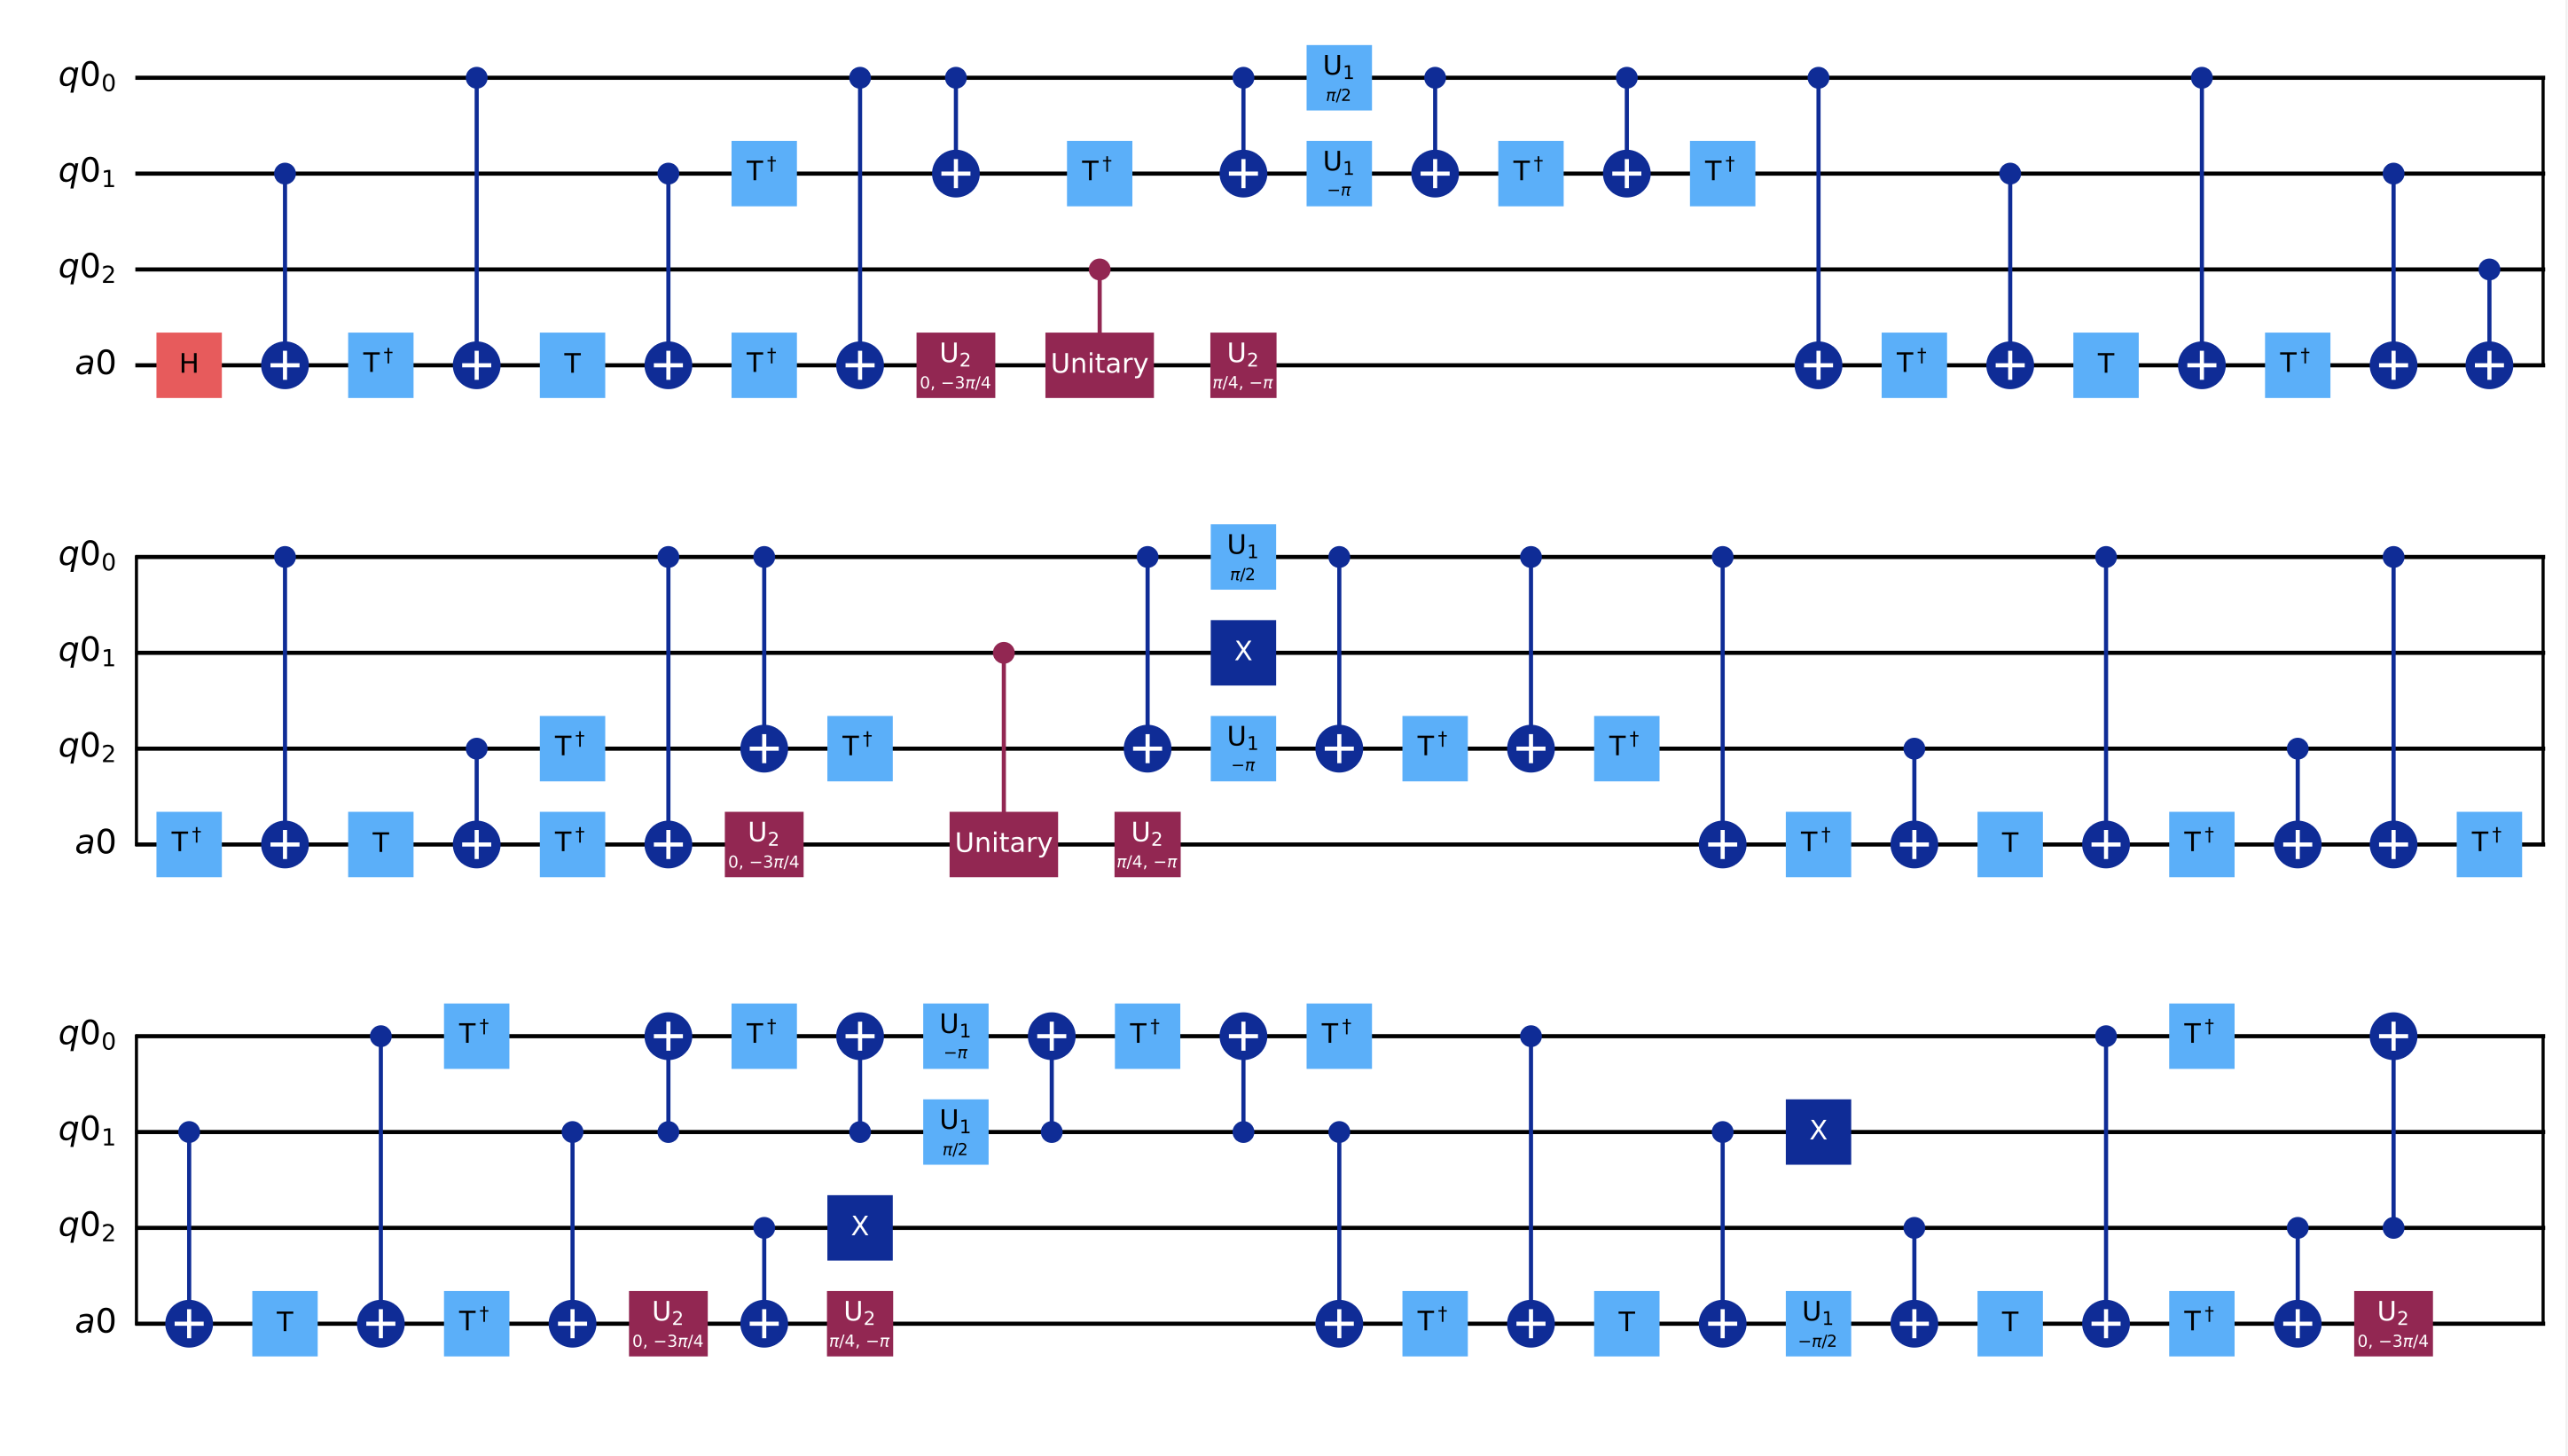
\includegraphics[width=0.45\textwidth]{circuit-example}}
        \caption{Compiled Qiskit circuit (partial) from cyclic permutation matrix.}
        \label{fig:cyclic-permute-circuit}
    \end{figure}
    The second example we are going to show is a little sophisticated.
    It's a randomly generated \(8 \times 8\) unitary matrix (group U(8)).
    We set the circuit decomposition granularity to \texttt{CTRL\_PRUNED} and the result has 1361 moments in Cirq.
    The compiled circuit is rendered in both Cirq and Qiskit as shown in~\ref{fig:unitary-compare}

    \begin{figure}[htbp]
        \centering
        \subfloat[Cirq circuit (partial)]{
            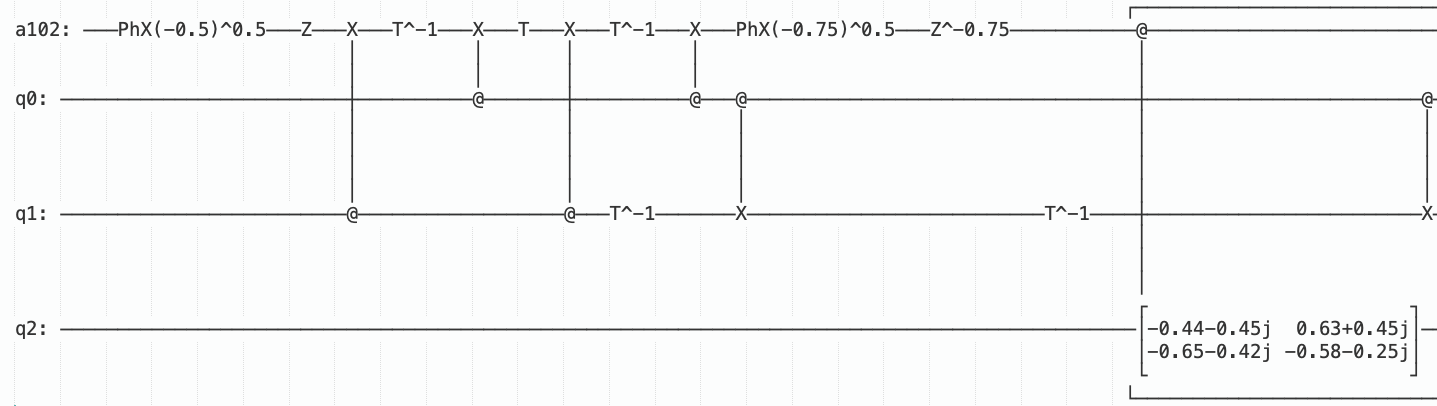
\includegraphics[width=0.45\textwidth]{cirq-unitary}
            \label{fig:cirq-unitary}
        }
        \hfill
        \subfloat[Qiskit circuit (partial)]{
            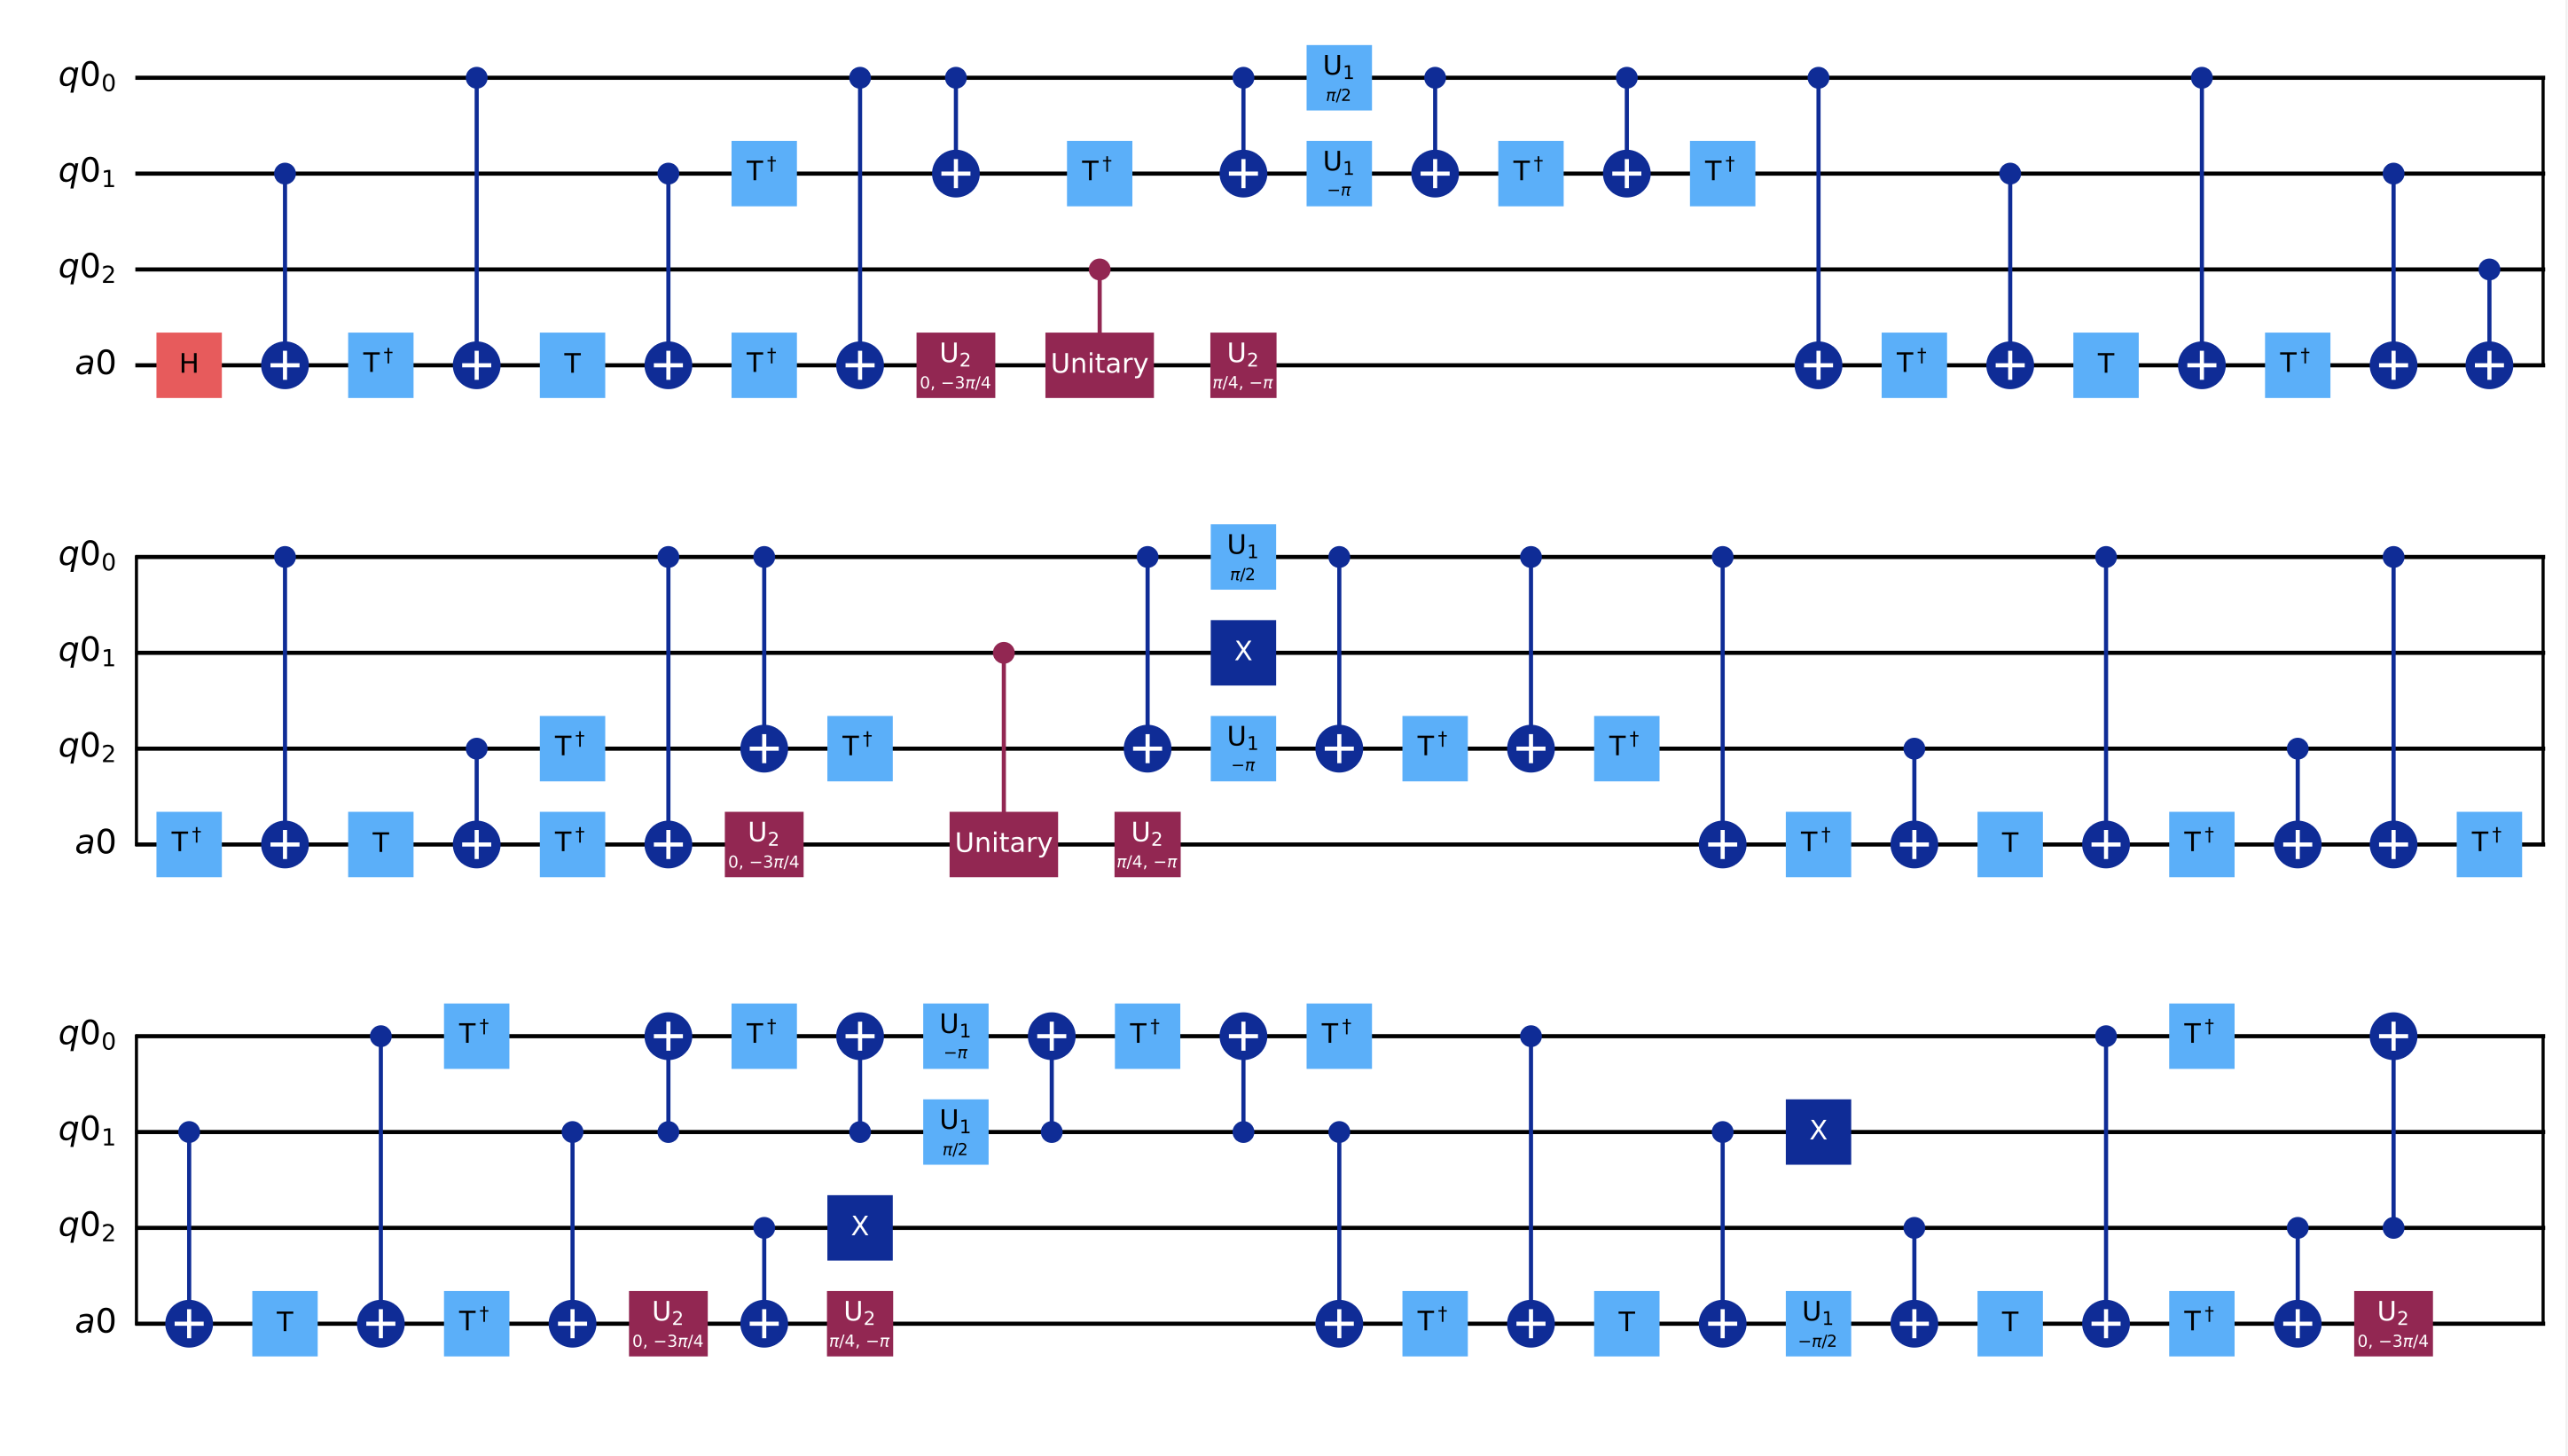
\includegraphics[width=0.45\textwidth]{circuit-example}
            \label{fig:qiskit-unitary}
        }
        \caption{An arbitary unitary matrix compiled once and rendered into both Cirq and Qiskit.}
        \label{fig:unitary-compare}
    \end{figure}


    \section{Conclusion and Future Work}\label{sec:conclusion-and-future-work}
    This poster proposal presents a cross-platform quantum compiler project that seeks to reduce platform friction in quantum software development.
    Future work includes:
    \begin{itemize}
        \item Integrating PennyLane and AWS Braket support
        \item Adding quantum error correction capability
    \end{itemize}
    We invite collaboration and feedback from the quantum software community.

    \begin{thebibliography}{00}
        \bibitem{nielsen2010quantum}
        M. A. Nielsen and I. L. Chuang, \textit{Quantum Computation and Quantum Information}, Cambridge Univ. Press, 2010.

        \bibitem{qiskit2023}
        H. Abraham, AduOffei, I. Y. Akhalwaya, et al.,
        “Qiskit: An open-source framework for quantum computing,”
        \textit{Zenodo}, 2023. doi: 10.5281/zenodo.2562111.

        \bibitem{cirq2024}
        Google Quantum AI, “Cirq,” 2024. [Online]. Available: \url{https://quantumai.google/cirq}

        \bibitem{braket-zenodo}
        Amazon Web Services, ``Amazon Braket SDK,'' Zenodo, 2023. [Online]. Available: \url{https://doi.org/10.5281/zenodo.4660670}

        \bibitem{pennylane}
        J. Bergholm \emph{et al.}, ``PennyLane: Automatic differentiation of hybrid quantum-classical computations,''
        \emph{arXiv preprint} arXiv:1811.04968, 2018. [Online]. Available: \url{https://arxiv.org/abs/1811.04968}

        \bibitem{dawson2005solovaykitaevalgorithm}
        C. M. Dawson and M. A. Nielsen, “The Solovay-Kitaev algorithm,”
        arXiv preprint quant-ph/0505030, 2005. [Online]. Available: \url{https://arxiv.org/abs/quant-ph/0505030}
    \end{thebibliography}

\end{document}
